% Resultados
\chapter{Pruebas experimentales} \label{sect:impresultados}

\section{Máquina de pruebas} \label{sect:testbed}

    Todas las pruebas fueron realizadas con un computador cuyas características
aparecen en la tabla \ref{tb:testbed}. El programa implementado, de nombre
{\bf mhs}, fue compilado con \emph{gcc} con optimización de nivel 3 en la
máquina mencionada anteriormente. Se eligió ese nivel de optimización ya que
aplica todas las mejoras del compilador \emph{gcc}.

\begin{table}[htb]
\footnotesize
\begin{center}
\begin{tabular}{|>{\columncolor{lightgray}}c|c|}
\hline
CPU & Intel Core I5 650 \\
\hline
RAM & 6 GB \\
\hline
Distribución & Ubuntu 11.04 x86\_64 bits \\
\hline
Kernel Linux & 2.6.38-8-generic \\
\hline
Versión gcc & 4.5.2 \\
\hline
\end{tabular}
\caption{Computador usado para las pruebas}
\label{tb:testbed}
\end{center}
\end{table}

\section{Formato de pruebas}  
\label{sect:ajustep}

    Se buscó el conjunto de mejores valores para los parámetros de cada algoritmo
implementado. Algunos de estos parámetros se mantuvieron fijos, decisión tomada
a partir de pruebas experimentales o recomendaciones de artículos y libros. Para
ello se realizaron dos conjuntos de pruebas y análisis:

\begin{enumerate}
    \item \emph{Pruebas con análisis de varianza}(ver apéndice \ref{apendiceb}):
            Para las pruebas, se recabó información de cada metaheurística de la
        siguiente forma:
        \begin{enumerate}
            \item Se generaron valores para el conjunto de parámetros de cada
        metaheurística, a partir de la permutación de rangos discretos válidos para cada
        uno de los mismos (véanse las secciones \ref{sect:iga-rv}, \ref{sect:iwpso-rv},
        \ref{sect:inpso-rv}, \ref{sect:inde-rv}, \ref{sect:isde-rv},
        \ref{sect:ibee-rv} y \ref{sect:iant-rv}).
            \item Se ejecutó cada metaheurística con cada uno de los conjunto de
        valores generados anteriormente y se extrajo el valor de la función de
        \emph{fitness} $f$ de cada solución final.
        \end{enumerate}
	\item \emph{Pruebas exhaustivas} (ver apéndice \ref{apendicea}):
            Para las pruebas, se recabó información de cada metaheurística de la
        siguiente forma:
        \begin{enumerate}
            \item Se generaron valores para el conjunto de parámetros de cada
        metaheurística a partir de la permutación de rangos discretos válidos para cada
        uno de los mismos (véanse las secciones  \ref{sect:agenetico}, \ref{sect:anpso},
        \ref{sect:awpso}, \ref{sect:ande}, \ref{sect:asde}, \ref{sect:abee},
        \ref{sect:aant}).
            \item Se ejecutó cinco veces cada metaheurística con cada uno de los     
        conjunto de valores generados anteriormente.
            \item De los resultados obtenidos, se promediaron las cinco corridas de cada
        metaheurística y se tomaron los veinte mejores conjunto de valores.
            \item Cada metaheurística fue ejecutada nuevamente con cada uno de los veinte
        mejores conjuntos de valores para ella. Fueron ejecutadas treinta veces para
        cada conjunto de valores.
        \end{enumerate}
\end{enumerate}

\subsection{Metaheurísticas híbridas}\label{exp:hibrido}

    Adicionalmente a la implementación de las metaheurísticas, también se implementaron
híbridos de éstas con el algoritmo determinista \emph{K-means}. En otras palabras,
las soluciones finales de cada metaheurística eran mejoradas por el algoritmo
\emph{K-means}.

    Se realizaron las \emph{pruebas exhaustivas} descritas anteriormente (ver
sección \ref{sect:ajustep}) tanto con las metaheurísticas híbridas como para las
no híbridas para luego hacer un análisis comparativo de las mismas (ver apéndice
\ref{apendicec}).

    Se utilizaron las metaheurísticas híbridas para hacer los análisis comparativos
del capítulo \ref{chap:analisis} ya que tuvieron mejor calidad de soluciones
finales que sus contrapartes no híbridas (ver apendice \ref{apendicec}).

\subsection{Archivos de prueba}\label{datatest}

    Las pruebas mencionadas anteriormente (ver sección \ref{sect:ajustep}) se
realizaron para los conjuntos de datos mostrados a continuación:
\begin{itemize}

\item {\bf Lenna:}\label{test:lenna} Es una imagen muy usada por los investigadores en el área 
de imágenes (ver figura
\subref{fig:lenna}). 
\textbf{El número óptimo de clusters está en el rango $[5,10]$\cite{OuBa2007}.}
Se usó una versión de resolución 128x128.

\item {\bf Iris:}\label{test:iris} Es un conjunto bastante conocido de datos que
consiste en tres diferentes especies de la planta iris: \emph{Iris setosa},
\emph{Iris virginica} e \emph{Iris versicolour}. Para cada una de las especies,
hay 50 muestras con cuatro atributos de tipo real: longitud del sépalo, ancho
del sépalo, longitud de pétalos y ancho de pétalos. \textbf{La partición óptima
es de 3 clusters con 50 objetos cada uno, de los cuales cada cluster representa a
una de las especies \cite{SwAjAm2008}.}

\item {\bf Imagen sintética:} Es una imagen creada con la finalidad de ver
gráficamente el buen funcionamiento
de las metaheurísticas implementadas (ver figura \subref{fig:Trivial}). \textbf{Al
ser una imagen simple, un buen
algoritmo debería encontrar la partición óptima (7 clusters: 6 figuras bien
diferenciadas y el fondo) sin ninguna dificultad.}

\end{itemize}

\begin{figure}[h!]
  \centering
  \subfloat[\emph{Lenna}]{\label{fig:lenna}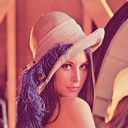
\includegraphics{figures/lenamini.png}} \qquad
  \subfloat[\emph{Imagen sintética}]{\label{fig:Trivial}
\includegraphics[scale=0.3]{figures/trivial.png}}
  \caption{Imágenes de prueba usadas}
  \label{fig:imgs}
\end{figure}

\subsection{Formato de las tablas de resultados}

    A continuación, se presentan los significados de las abreviaturas de las
cabeceras de las tablas de resultados:
\begin{itemize}
    \item \textbf{FO}: Valor de la función de \emph{fitness} $1/DB$ para la
solución final.
    \item \textbf{DB}: Valor del índice \emph{DB} para la solución final.
    \item \textbf{$J_e$}: Valor de la cuantificación del error para la solución
final.
	\item \textbf{E}:Cantidad de evaluaciones de la función de \emph{fitness}.
\end{itemize}

\section{Resultados del K-means}

    En esta sección, se muestran los resultados del algoritmo determinista
\emph{K-means}.

\subsection{Resultados obtenidos para \textbf{Lenna}}

    A continuación, se presenta una tabla resumen de 30 ejecuciones del
algoritmo \emph{K-means} con la imagen \textbf{Lenna}:

\begin{table}[h!]
\footnotesize
\begin{center}
\begin{tabular}{|c|c|c|c|c|}
\hline
&{\bf FO}&{\bf DB}&{\bf $J_e$}\\
\hline
\hline
Promedio & 1.2037 & 0.8333 & 17.1739\\
\hline
Mejor & 1.2797 & 0.7814 & 16.9164\\
\hline
Peor & 1.0456 & 0.9564 & 17.091\\
\hline
\end{tabular}
\caption{Resultados de \emph{K-means} para {\bf Lenna}}
\label{tb:pmpkmeansimg}
\end{center}
\end{table}


\subsection{Resultados obtenidos para \textbf{Iris}}

    A continuación, se presenta una tabla resumen de 30 ejecuciones del
algoritmo \emph{K-means} con el archivo de datos numéricos \textbf{Iris}:

\begin{table}[h!]
\footnotesize
\begin{center}
\begin{tabular}{|c|c|c|c|c|}
\hline
&{\bf FO}&{\bf DB}&{\bf $J_e$}\\
\hline
\hline
Promedio & 1.4915 & 0.6756 & 0.64\\
\hline
Mejor & 1.6695 & 0.599 & 0.6339\\
\hline
Peor & 0.9983 & 1.0017 & 0.7094\\
\hline
\end{tabular}
\caption{Resultados de \emph{K-means} para {\bf Lenna}}
\label{tb:pmpkmeanscsv}
\end{center}
\end{table}


\section{Resultados del \emph{GA}}

    En esta sección, se muestran los resultados del algoritmo genético híbrido con
\emph{K-means} (\emph{GAH}) para la imagen \textbf{Lenna} y el archivo de datos
numéricos \textbf{Iris} (ver sección \ref{exp:hibrido}).

\subsection{Parámetros variables}\label{sect:iga-pv}

    A continuación, se describen los parámetros variables del algoritmo:
\begin{itemize}
    \item $I$: representa a la cantidad total de individuos de la población,
donde $I \geq 2$.
    \item $tt$: representa el tamaño del torneo, donde $tt \geq 2$ y $tt \leq I$.
    \item $pc$: representa la probabilidad de cruce de los individuos y
está acotado en el rango $[0, 1]$.
    \item $pm$: representa la probabilidad de mutación de los individuos y
está acotado en el rango $[0, 1]$.
\end{itemize}

\subsubsection{Resultados obtenidos para \textbf{Lenna}}

    A continuación, se presenta una tabla resumen de 30 ejecuciones del mejor
conjunto de valores para los parámetros del algoritmo \emph{GAH}:

\begin{table}[h!]
\footnotesize
\begin{center}
\begin{tabular}{|c|c|c|c|c|c|c|c|c|c|}
\hline
& {\bf FO} & {\bf DB}& $J_e$ & $I$ & $tt$ & $pc$ & $pm$ \\
\hline
\hline
Promedio   & 1.2753 & 0.7853  & 17.5582 &  &  &  & \\
\cline{1-4}
Mejor & 1.4104 & 0.709  & 19.4009 & 10 & 4 & 0.8 & 1.0\\
\cline{1-4}
Peor & 1.179 & 0.8481  & 17.6034 &  &  &  & \\\hline
\end{tabular}
\caption{Resultados de las mejores corridas de \emph{GAH} para {\bf Lenna}}
\label{tb:pmpgahibimg}
\end{center}
\end{table}


\subsubsection{Resultados obtenidos para \textbf{Iris}}

    A continuación, se presenta una tabla resumen de 30 ejecuciones del mejor
conjunto de valores para los parámetros del algoritmo \emph{GAH}:

\begin{table}[h!]
\footnotesize
\begin{center}
\begin{tabular}{|c|c|c|c|c|c|c|c|c|c|}
\hline
& {\bf FO} & {\bf DB}& $J_e$ & $I$ & $tt$ & $pc$ & $pm$ \\
\hline
\hline
Promedio   & 2.6521 & 0.3771  & 0.5029 &  &  &  & \\
\cline{1-4}
Mejor & 2.6521 & 0.3771  & 0.5029 & 25 & 12 & 0.2 & 1.0\\
\cline{1-4}
Peor & 2.6521 & 0.3771  & 0.5029 &  &  &  & \\\hline
\end{tabular}
\caption{Resultados de las mejores corridas de \emph{GAH} para {\bf Iris}}
\label{tb:pmpgahibcsv}
\end{center}
\end{table}


\subsubsection{Influencia de los parámetros}

Teniendo en cuenta que el \emph{rango probado} es el conjunto de valores utilizado
para las pruebas y el \emph{rango efectivo} es el conjunto valores de los parámetros
para los 20 mejores resultados del algoritmo \emph{GAH} (tablas \ref{tb:tablegahibimg}
y \ref{tb:tablegahibcsv}), se encontró lo siguiente:

\begin{itemize}
    \item Para la imagen \textbf{Lenna}:
        \begin{itemize}
            \item Parámetro $I$:
                Como el \emph{rango probado} ($[5, 40]$) es
                igual al \emph{rango efectivo} ($[5, 40]$) no importa que valor tome el
                parámetro $I$, el \emph{GAH} puede dar una buena solución
                final. Por lo tanto, este parámetro no influye
                considerablemente en la bondad de la solución final.
            \item Parámetro $tt$:
                Como el \emph{rango probado}($[4, 40]$) es
                mayor al \emph{rango efectivo} ($[4, 24]$), es relevante el valor que se
                le asigne al parámetro $tt$. \textbf{Por lo tanto, este
                parámetro influye en la bondad de la solución final.}
            \item Parámetro $pc$:
                Como el \emph{rango probado}($[0.0; 1.0]$) es
                practicamente igual al \emph{rango efectivo} (sólo faltan el $0.4$ y $0.9$), 
                no importa que valor tome el
                parámetro $pc$, el \emph{GAH} puede dar una buena solución
                final. Por lo tanto, este parámetro no influye
                considerablemente en la bondad de la solución final.
            \item Parámetro $pm$:
                Como el \emph{rango probado}($[0.1; 1.0]$ ) es
                mayor al \emph{rango efectivo} ($[0.5; 1.0]$ ), es relevante el valor que se
                le asigne al parámetro $pm$. \textbf{Por lo tanto, este
                parámetro influye en la bondad de la solución final.}
        \end{itemize}
	\item Para el archivo numérico \textbf{Iris}:
        \begin{itemize}
            \item Parámetro $I$:
                Como el \emph{rango probado}($[5, 40]$) es
                mayor al \emph{rango efectivo} ($[25, 40]$), es relevante el valor que se
                le asigne al parámetro $I$. \textbf{Por lo tanto, este
                parámetro influye en la bondad de la solución final.}
			\item Para los parámetros $tt$, $pc$ y $pm$ se observa un comportamiento
				similar al encontrado para la imagen \textbf{Lenna}.
        \end{itemize}
\end{itemize}

\section{Resultados del \emph{WPSO}}

    En esta sección, se muestran los resultados de la metaheurística \emph{WPSO}
híbrida con \emph{K-means} (\emph{WPSOH\-}) para la imagen \textbf{Lenna}
y el archivo de datos numéricos \textbf{Iris} (ver sección \ref{exp:hibrido}).

\subsection{Parámetros variables}\label{sect:iwpso-pv}

    A continuación, se describen los parámetros variables del algoritmo:
\begin{itemize}
    \item $I$: representa a la cantidad total de partículas del enjambre,
donde $I \geq 2$.
    \item $w_1$, $w_2$ y $w_3$: son los pesos de la función de \emph{fitness}
(\ref{pso: wpso}), deben ser positivos y su suma debe ser igual a 1.
    \item $W$, $c_1$ y $c_2$: representan al peso inercial, factor de aprendizaje
colectivo y factor de aprendizaje social, respectivamente, descritos en la
sección \ref{sect:metapso-vel}. $W$ debe estar acotado en el rango $[0, 2]$ y
$c_1$ y $c_2$ deben satisfacer la inecuación (\ref{pso: convergece}).
    \item $vmx$: es un escalar, acotado en el rango $[0, 1]$, que multiplica al
vector $Z_{max}$ con el fin de regular la velocidad máxima de la partícula,
donde $vmx \cdot Z_{max}$ es el valor máximo de la velocidad $v(t)$ (véase la
ecuación (\ref{pso: vi})).
\end{itemize}

\subsubsection{Resultados obtenidos para \textbf{Lenna}}
    A continuación, se presenta una tabla resumen de 30 ejecuciones del mejor
conjunto de valores para los parámetros del algoritmo \emph{WPSOH}:

\begin{table}[h!]
\footnotesize
\begin{center}
\begin{tabular}{|c|c|c|c|c|c|c|c|c|c|c|c|c|c|}
\hline
& {\bf FO} & {\bf DB}& $J_e$ & $I$ & $w_1$ & $w_2$ & $w_3$ & $W$ & $c_1$ & $c_2$ & $vmx$ \\
\hline
\hline
Promedio   & 1.2005 & 0.8348  & 17.7634 &  &  &  &  &  &  &  & \\
\cline{1-4}
Mejor & 1.3039 & 0.7669  & 16.9839 & 35 & 0.0 & 1.0 & 0.0 & 0.5 & 2.0 & 0.5 & 0.5\\
\cline{1-4}
Peor & 1.1074 & 0.903  & 17.6885 &  &  &  &  &  &  &  & \\\hline
\end{tabular}
\caption{Resultados de las mejores corridas de \emph{WPSOH} para {\bf Lenna}}
\label{tb:pmpwpsohibimg}
\end{center}
\end{table}


\subsubsection{Resultados obtenidos para \textbf{Iris}}

    A continuación, se presenta una tabla resumen de 30 ejecuciones del mejor
conjunto de valores para los parámetros del algoritmo \emph{WPSOH}:

\begin{table}[h!]
\footnotesize
\begin{center}
\begin{tabular}{|c|c|c|c|c|c|c|c|c|c|c|c|c|c|}
\hline
& {\bf FO} & {\bf DB}& $J_e$ & $I$ & $w_1$ & $w_2$ & $w_3$ & $W$ & $c_1$ & $c_2$ & $vmx$ \\
\hline
\hline
Promedio   & 1.5694 & 0.6385  & 0.661 &  &  &  &  &  &  &  & \\
\cline{1-4}
Mejor & 1.6992 & 0.5885  & 0.6709 & 10 & 0.8 & 0.2 & 0.0 & 0.8 & 1.1 & 1.1 & 0.5\\
\cline{1-4}
Peor & 1.5165 & 0.6594  & 0.6466 &  &  &  &  &  &  &  & \\\hline
\end{tabular}
\caption{Resultados de las mejores corridas de \emph{WPSOH} para {\bf Iris}}
\label{tb:pmpwpsohibcsv}
\end{center}
\end{table}


\subsubsection{Influencia de los parámetros}

Teniendo en cuenta que el \emph{rango probado} es el conjunto de valores utilizado
para las pruebas y el \emph{rango efectivo} es el conjunto valores de los parámetros
para los 20 mejores resultados del algoritmo \emph{WPSOH} (tablas \ref{tb:tablewpsohibimg}
y \ref{tb:tablewpsohibcsv}), se encontró lo siguiente:

\begin{itemize}
	\item Para la imagen \textbf{Lenna}:
	\begin{itemize}
		\item No se puede encontrar una relación entre los valores de los
			parámetros y el valor de la función de \emph{fitness}. Se
			puede observar que para cada parámetro el \emph{rango efectivo}
			es similar \emph{rango probado}. Esto indica que el valor que tome cada
			uno de los parámetros del algoritmo parece no tener una gran influencia en la
			solución final.
	\end{itemize}
	\item Para el archivo numérico \textbf{Iris}:
	\begin{itemize}
		\item Se puede observar que los parámetros $I$, $w_1$, $w_2$, $w_3$ y
			$W$ pueden ser fijados en $10$, $0.8$, $0.2$, $0.0$ y $0.8$,
			respectivamente. Los demás parámetros se comportan de manera similar 
			a como lo hacen para la imagen {\bf Lenna}.
	\end{itemize}
\end{itemize}

\section{Resultados del \emph{NPSO}}

    En esta sección, se muestran los resultados de la metaheurística \emph{NPSO}
híbrida con \emph{K-means} (\emph{NPSOH}) para la imagen \textbf{Lenna} y el archivo
de datos numéricos \textbf{Iris} (ver sección \ref{exp:hibrido}).

\subsection{Parámetros variables}\label{sect:inpso-pv}

    Los parámetros variables son los mismos descritos en la sección \ref{sect:iwpso-pv},
exceptuando los pesos $w_1$, $w_2$ y $w_3$.

\subsubsection{Resultados obtenidos para \textbf{Lenna}}

    A continuación, se presenta una tabla resumen de 30 ejecuciones del mejor
conjunto de valores para los parámetros del algoritmo \emph{NPSOH}:

\begin{table}[h!]
\footnotesize
\begin{center}
\begin{tabular}{|c|c|c|c|c|c|c|c|c|c|c|}
\hline
& {\bf FO} & {\bf DB}& $J_e$ & $I$ & W & $c_1$ & $c_2$ & $vmx$ \\
\hline
\hline
Promedio   & 1.2071 & 0.8297  & 17.5799 & &  &  &  & \\
\cline{1-4}
Mejor & 1.2968 & 0.7711  & 17.3749 & 35 & 0.8 & 1.7 & 1.7 & 0.5\\
\cline{1-4}
Peor & 1.1113 & 0.8999  & 19.3463 &  &  &  &  & \\\hline
\end{tabular}
\caption{Resultados de las mejores corridas de \emph{NPSOH} para {\bf Lenna}}
\label{tb:pmppsohibimg}
\end{center}
\end{table}


\subsubsection{Resultados obtenidos para \textbf{Iris}}

    A continuación, se presenta una tabla resumen de 30 ejecuciones del mejor
conjunto de valores para los parámetros del algoritmo \emph{NPSOH}:

\begin{table}[h!]
\footnotesize
\begin{center}
\begin{tabular}{|c|c|c|c|c|c|c|c|c|c|c|}
\hline
& {\bf FO} & {\bf DB}& $J_e$ & $I$ & W & $c_1$ & $c_2$ & $vmx$ \\
\hline
\hline
Promedio   & 1.5654 & 0.6395  & 0.6606 &  &  &  &  & \\
\cline{1-4}
Mejor & 1.6626 & 0.6015  & 0.6807 & 25 & 1.1 & 1.7 & 0.5 & 0.5\\
\cline{1-4}
Peor & 1.5006 & 0.6664  & 0.649 &  &  &  &  & \\\hline
\end{tabular}
\caption{Resultados de las mejores corridas de \emph{NPSOH} para {\bf Iris}}
\label{tb:pmppsohibcsv}
\end{center}
\end{table}


\subsubsection{Influencia de los parámetros}

Teniendo en cuenta que el \emph{rango probado} es el conjunto de valores utilizado
para las pruebas y el \emph{rango efectivo} es el conjunto valores de los parámetros
para los 20 mejores resultados del algoritmo \emph{NPSOH} (tablas \ref{tb:tablepsohibimg}
y \ref{tb:tablepsohibcsv}), se encontró lo siguiente:

\begin{itemize}
	\item Para la imagen \textbf{Lenna}:
	\begin{itemize}
		\item No se puede encontrar una relación entre los valores de los
			parámetros y el valor de la función de \emph{fitness}. Se
			puede observar que para cada parámetro el \emph{rango efectivo}
			es similar \emph{rango probado}. Esto indica que el valor que tome cada
			uno de los parámetros del algoritmo parece no tener una gran influencia en la
			solución final.
	\end{itemize}
	\item Para el archivo numérico \textbf{Iris}:
	\begin{itemize}
		\item Se puede observar que los parámetros $I$ y $W$ pueden ser fijados
			en $25$ y $1.1$, respectivamente. Los demás parámetros se comportan de manera similar 
			a como lo hacen para la imagen {\bf Lenna}.
	\end{itemize}
\end{itemize}

\section{Resultados del \emph{SDE}}

    En esta sección, se muestran los resultados de la metaheurística  \emph{SDE}
híbrida con \emph{K-means} (\emph{SDEH}) para la imagen \textbf{Lenna} y el
archivo de datos numéricos \textbf{Iris} (ver sección \ref{exp:hibrido}).

\subsection{Parámetros variables}\label{sect:isde-pv}

    A continuación, se describen los parámetros variables del algoritmo:
\begin{itemize}
    \item $I$: representa a la cantidad total de individuos, donde $I \geq 4$.
    \item $w_1$, $w_2$ y $w_3$: son los pesos de la función de \emph{fitness}
(\ref{pso: wpso}), deben ser positivos y su suma debe ser igual a 1.
    \item $\gamma$: factor de escalados de la diferencia. Está acotado en el rango $[0, 1]$.
    \item $Cr$: representa la probabilidad de cruce  de los individuos y
está acotado en el rango $[0, 1]$.
\end{itemize}

\subsubsection{Resultados obtenidos para \textbf{Lenna} (\emph{SDEH})}

    A continuación, se presenta una tabla resumen de 30 ejecuciones del mejor
conjunto de valores para los parámetros del algoritmo \emph{SDEH}:

\begin{table}[h!]
\footnotesize
\begin{center}
\begin{tabular}{|c|c|c|c|c|c|c|c|c|c|c|c|}
\hline
& {\bf FO} & {\bf DB}& $J_e$ & $I$ & $w_1$ & $w_2$ & $w_3$ & $\gamma$ & $Cr$ \\
\hline
\hline
Promedio   & 1.1813 & 0.8491  & 19.5178 &  &  &  &  &  & \\
\cline{1-4}
Mejor & 1.3195 & 0.7578  & 16.9559 & 10 & 0.4 & 0.5 & 0.1 & 0.5 & 0.7\\
\cline{1-4}
Peor & 0.9948 & 1.0052  & 39.0413 &  &  &  &  &  & \\\hline
\end{tabular}
\caption{Resultados de las mejores corridas de \emph{SDEH} para {\bf Lenna}}
\label{tb:pmpsdehibimg}
\end{center}
\end{table}


\subsubsection{Resultados obtenidos para \textbf{Iris} (\emph{SDEH})}

    A continuación, se presenta una tabla resumen de 30 ejecuciones del mejor
conjunto de valores para los parámetros del algoritmo \emph{SDEH}:

\begin{table}[h!]
\footnotesize
\begin{center}
\begin{tabular}{|c|c|c|c|c|c|c|c|c|c|c|c|}
\hline
& {\bf FO} & {\bf DB}& $J_e$ & $I$ & $w_1$ & $w_2$ & $w_3$ & $\gamma$ & $Cr$ \\
\hline
\hline
Promedio   & 1.5312 & 0.6533  & 0.6448 &  &  &  &  &  & \\
\cline{1-4}
Mejor & 1.5778 & 0.6338  & 0.625 & 15 & 0.5 & 0.1 & 0.4 & 0.8 & 0.9\\
\cline{1-4}
Peor & 1.5006 & 0.6664  & 0.649 &  &  &  &  &  & \\\hline
\end{tabular}
\caption{Resultados de las mejores corridas de \emph{SDEH} para {\bf Iris}}
\label{tb:pmpsdehibcsv}
\end{center}
\end{table}


\subsubsection{Influencia de los parámetros}

Teniendo en cuenta que el \emph{rango probado} es el conjunto de valores utilizado
para las pruebas y el \emph{rango efectivo} es el conjunto valores de los parámetros
para los 20 mejores resultados del algoritmo \emph{SDEH} (tablas \ref{tb:tablesdehibimg}
y \ref{tb:tablesdehibcsv}), se encontró lo siguiente:

\begin{itemize}
    \item Para la imagen {\bf Lenna}:
		\begin{itemize}
		    \item Para los parámetros $I$, $w_1$ y $w_3$ el \emph{rango efectivo}
				  es similar \emph{rango probado}. Esto
				  puede indicar que no influyen considerablemente en la calidad
				  de las soluciones finales.
		    \item Para los parámetros $\gamma$ y $Cr$  el \emph{rango efectivo} 
		          posee una gran cantidad de valores del \emph{rango probado}.
		          Esto puede indicar que no influyen considerablemente en la
		          calidad de las soluciones finales.
		    \item Parámetro $w_2$:
		          Como el \emph{rango probado}($[0.1; 1.0]$) es
		          mayor al \emph{rango efectivo} ($[0.0;0.8]$), es relevante el valor que se
		          le asigne al parámetro $w_2$. \textbf{Por lo tanto, este
		          parámetro influye en la bondad de la solución final.}
	    \end{itemize}
    
    \item Para el archivo numérico {\bf Iris}:
		\begin{itemize}
			\item Se puede observar que los parámetros $I$, $w_1$, $w_2$ y $w_3$
			  	  pueden ser fijados en  $15$, $0.5$, $0.1$ y $0.4$,
				  respectivamente. 
		    \item Parámetro $\gamma$:
		          Como el \emph{rango probado}($[0.5; 1.0]$) es
		          mayor al \emph{rango efectivo} ($[0.5;0.8]$), es relevante el valor que se
		          le asigne al parámetro $\gamma$. Además, mientras más alto
		          sea su valor, mejor es el valor de la función de \emph{fitness}.
		           \textbf{Por lo tanto, este
		          parámetro influye en la bondad de la solución final.}
		    \item Parámetro $Cr$:
		    	  Tiene un comportamiento similar al obtenido con \textbf{Lenna}.
		\end{itemize}
\end{itemize}

\section{Resultados del \emph{NDE}}

    En esta sección, se muestran los resultados de la metaheurística \emph{NDE}
híbrido con \emph{K-means} (\emph{NDEH}) para la imagen \textbf{Lenna} y el
archivo de datos numéricos \textbf{Iris} (ver sección \ref{exp:hibrido}).

\subsection{Parámetros variables}\label{sect:inde-pv}

    Los parámetros son los mismos que para el algoritmo \emph{SDEH} (ver la sección
\ref{sect:isde-pv}). Sin embargo, se calculan automáticamente los parámetros
$\gamma$ y $Cr$.

\subsubsection{Resultados obtenidos para \textbf{Lenna} (\emph{NDEH})}

    A continuación, se presenta una tabla resumen de 30 ejecuciones del mejor
conjunto de valores para los parámetros del algoritmo \emph{NDEH}:

\begin{table}[h!]
\footnotesize
\begin{center}
\begin{tabular}{|c|c|c|c|c|c|c|c|c|c|}
\hline
& {\bf FO} & {\bf DB}& $J_e$ & $I$ & $w_1$ & $w_2$ & $w_3$ \\
\hline
\hline
Promedio   & 1.2132 & 0.8256  & 19.9024 &  &  &  & \\
\cline{1-4}
Mejor & 1.3346 & 0.7493  & 16.589 & 40 & 0.0 & 0.0 & 1.0\\
\cline{1-4}
Peor & 1.1097 & 0.9011  & 17.6334 &  &  &  & \\\hline
\end{tabular}
\caption{Resultados de las mejores corridas de \emph{NDEH} para {\bf Lenna}}
\label{tb:pmpdehibimg}
\end{center}
\end{table}


\subsubsection{Resultados obtenidos para \textbf{Iris} (\emph{NDEH})}

    A continuación, se presenta una tabla resumen de 30 ejecuciones del mejor
conjunto de valores para los parámetros del algoritmo \emph{NDEH}:

\begin{table}[h!]
\footnotesize
\begin{center}
\begin{tabular}{|c|c|c|c|c|c|c|c|c|c|}
\hline
& {\bf FO} & {\bf DB}& $J_e$ & $I$ & $w_1$ & $w_2$ & $w_3$ \\
\hline
\hline
Promedio   & 1.5638 & 0.6403  & 0.6367 &  &  &  & \\
\cline{1-4}
Mejor & 1.7153 & 0.583  & 0.6586 & 15 & 0.2 & 0.7 & 0.1\\
\cline{1-4}
Peor & 1.5006 & 0.6664  & 0.649 &  &  &  & \\\hline
\end{tabular}
\caption{Resultados de las mejores corridas de \emph{NDEH} para {\bf Iris}}
\label{tb:pmpdehibcsv}
\end{center}
\end{table}


\subsubsection{Influencia de los parámetros}

Teniendo en cuenta que el \emph{rango probado} es el conjunto de valores utilizado
para las pruebas y el \emph{rango efectivo} es el conjunto valores de los parámetros
para los 20 mejores resultados del algoritmo \emph{NDEH} (tablas \ref{tb:tabledehibimg}
y \ref{tb:tabledehibcsv}), se encontró lo siguiente:

\begin{itemize}
    \item Para la imagen {\bf Lenna}:
		\begin{itemize}
		    \item Para los parámetros $I$, $w_1$ y $w_3$ el \emph{rango efectivo}
				  es similar \emph{rango probado}. Esto
		          puede indicar que no influyen considerablemente en la calidad
		          de las soluciones finales.
		    \item Parámetro $w_2$:
		          Como el \emph{rango probado}($[0.1; 1.0]$) es
		          mayor al \emph{rango efectivo} ($[0.0;0.6]$), es relevante el valor que se
		          le asigne al parámetro $w_2$. \textbf{Por lo tanto, este
		          parámetro influye en la bondad de la solución final.}
		\end{itemize}
    \item Para el archivo numérico {\bf Iris}:
		\begin{itemize}
		    \item A diferencia de los resultados para \emph{Lenna}, ningún
		    parámetro parece influir considerablemente en la calidad de las
		    soluciones finales.
		\end{itemize}
\end{itemize}

\section{Resultados del \emph{Bee}}

    En esta sección, se muestran los resultados del algoritmo de abeja híbrido con
\emph{K-means} (\emph{BeeH}) para la imagen \textbf{Lenna} y el archivo de datos
numéricos \textbf{Iris} (ver sección \ref{exp:hibrido}).

\subsection{Parámetros variables}\label{sect:ibee-pv}

    A continuación, se describen los parámetros variables del algoritmo:
\begin{itemize}
    \item $I$: Representa a la cantidad total de abejas del enjambre,
donde $I \geq 2$.
    \item $m$: Representa los sitios de flores totales, donde $m < I$.
    \item $e$: Representa los sitios de flores élite, donde $e < m$.
    \item $eb$ y $ob$: Representan la cantidad de abejas élite y la cantidad de
abejas exploradoras, respectivamente, donde $eb + ob \leq I$.
\end{itemize}

\subsubsection{Resultados obtenidos para \textbf{Lenna}}

    A continuación, se presenta una tabla resumen de 30 ejecuciones del mejor
conjunto de valores para los parámetros del algoritmo \emph{BeeH}:

\begin{table}[h!]
\footnotesize
\begin{center}
\begin{tabular}{|c|c|c|c|c|c|c|c|c|c|c|}
\hline
& {\bf FO} & {\bf DB}& $J_e$ & $I$ & $m$ & $e$ & $eb$ & $ob$ \\
\hline
\hline
Promedio   & 1.3052 & 0.7664  & 16.924 &  &  &  &  & \\
\cline{1-4}
Mejor & 1.3624 & 0.734  & 16.9922 & 35 & 15 & 2 & 14 & 6\\
\cline{1-4}
Peor & 1.2586 & 0.7945  & 16.7638 &    &  &  &  & \\\hline
\end{tabular}
\caption{Resultados de las mejores corridas de \emph{BeeH} para {\bf Lenna}}
\label{tb:pmpbeehibimg}
\end{center}
\end{table}


\pagebreak

\subsubsection{Resultados obtenidos para \textbf{Iris}}

    A continuación, se presenta una tabla resumen de 30 ejecuciones del mejor
conjunto de valores para los parámetros del algoritmo \emph{BeeH}:

\begin{table}[h!]
\footnotesize
\begin{center}
\begin{tabular}{|c|c|c|c|c|c|c|c|c|c|c|}
\hline
& {\bf FO} & {\bf DB}& $J_e$ & $I$ & $m$ & $e$ & $eb$ & $ob$ \\
\hline
\hline
Promedio   & 1.9167 & 0.5412  & 0.6281 &  &  &  &  & \\
\cline{1-4}
Mejor & 2.6521 & 0.3771  & 0.5029 & 30 & 15 & 12 & 6 & 9\\
\cline{1-4}
Peor & 1.6451 & 0.6079  & 0.6287 &  &  &  &  & \\\hline
\end{tabular}
\caption{Resultados de las mejores corridas de \emph{BeeH} para {\bf Iris}}
\label{tb:pmpbeehibcsv}
\end{center}
\end{table}


\subsubsection{Influencia de los parámetros}

Teniendo en cuenta que el \emph{rango probado} es el conjunto de valores utilizado
para las pruebas y el \emph{rango efectivo} es el conjunto valores de los parámetros
para los 20 mejores resultados del algoritmo \emph{BeeH} (tablas \ref{tb:tablebeehibimg}
y \ref{tb:tablebeehibcsv}), se encontró lo siguiente:

\begin{itemize}
        \item Para la imagen {\bf Lenna}:
	        \begin{itemize}
		        \item Parámetro $I$:
		            Como el \emph{rango probado} ($[5, 40]$) es
		            mayor al \emph{rango efectivo} ($[25, 40]$) , es relevante el valor que se
		            le asigne al parámetro $I$. \textbf{Por lo tanto, este
		            parámetro influye en la bondad de la solución final.}
		            considerablemente en la bondad de la solución final.
		        \item Parámetro $m$:
		        	Es mayor o igual a 7,
					aunque la mayor parte de los datos se encuentra en el rango $[11, 15]$.
					De tal forma el \emph{rango probado} ($[5, 15]$) es
		            mayor al \emph{rango efectivo}, generando que sea relevante el valor que se
		            le asigne al parámetro $m$. \textbf{Por lo tanto, este
		            parámetro influye en la bondad de la solución final.}
		        \item Parámetro $e$:
		            Como el \emph{rango probado}($[1,15]$) es
		            mayor al \emph{rango efectivo} ($[1,5]$), es relevante el valor que se
		            le asigne al parámetro $e$. \textbf{Por lo tanto, este
		            parámetro influye en la bondad de la solución final.}
		        \item Parámetro $eb$:
					Está en el rango $[10, 15]$, con ciertas excepciones.
					De tal forma el \emph{rango probado} ($[5, 15]$) es
		            mayor al \emph{rango efectivo}, generando que sea relevante el valor que se
		            le asigne al parámetro $eb$. Lo cual indica que con
					una cantidad de abejas élite menor a 10, la solución final tiende a desmejorar.
					\textbf{Por lo tanto, este parámetro influye en la bondad de la solución final.} 
		        \item Parámetro $ob$:
		            Como el \emph{rango probado}($[1,15]$) es
		            practicamente igual al \emph{rango efectivo} (sólo faltan el $3$, $10$, $11$ y $14$), 
		            no importa que valor tome el
		            parámetro $pc$, el \emph{BeeH} puede dar una buena solución
		            final. Por lo tanto, este parámetro no influye
		            considerablemente en la bondad de la solución final.
            \end{itemize}
        \item Para el archivo numérico {\bf Iris}:
		    \begin{itemize}
		        \item Los parámetros $I$, $m$, $e$ y $ob$ conservan el mismo comportamiento
					  que para la imagen \textbf{Lenna}. Sin embargo, el parámetro $eb$ no parece
					  mostrar el mismo patrón mostrado para las corridas de la imagen. Por lo tanto,
				  	  es posible que el valor de $eb$ no tenga tanta influencia en la bondad de la
					  solución final para el archivo numérico \textbf{Iris}.
		    \end{itemize}
\end{itemize}

\section{Resultados del \emph{Ant}}

    En esta sección, se muestran los resultados del algoritmo de hormia híbrido con
\emph{K-means} (\emph{AntH}) para la imagen \textbf{Lenna} y el archivo de datos
numéricos \textbf{Iris} (ver sección \ref{exp:hibrido}).

\subsection{Parámetro variable}\label{sect:iant-pv}

    A continuación, se describe el parámetro variable del algoritmo:
\begin{itemize}
    \item $I$: representa a la cantidad total de hormigas, donde $I \geq 2$.
\end{itemize}

\subsubsection{Resultados obtenidos para \textbf{Lenna}}

    A continuación, se presenta una tabla resumen de 30 ejecuciones del mejor
conjunto de valores para los parámetros del algoritmo \emph{AntH}:

\begin{table}[h!]
\footnotesize
\begin{center}
\begin{tabular}{|c|c|c|c|c|c|c|}
\hline
& {\bf FO} & {\bf DB}& $J_e$ & $I$\\
\hline
\hline
Promedio   & 1.0581 & 0.9483  & 11.4482 & \\
\cline{1-4}
Mejor & 1.2015 & 0.8323  & 11.2246 & 40\\
\cline{1-4}
Peor & 0.9367 & 1.0676  & 9.8267 & \\\hline
\end{tabular}
\caption{Resultados de las mejores corridas de \emph{AntH} para {\bf Lenna}}
\label{tb:pmpanthibimg}
\end{center}
\end{table}


\pagebreak

\subsubsection{Resultados obtenidos para \textbf{Iris}}

    A continuación, se presenta una tabla resumen de 30 ejecuciones del mejor
conjunto de valores para los parámetros del algoritmo \emph{AntH}:

\begin{table}[h!]
\footnotesize
\begin{center}
\begin{tabular}{|c|c|c|c|c|c|c|}
\hline
& {\bf FO} & {\bf DB}& $J_e$ & $I$\\
\hline
\hline
Promedio   & 1.053 & 0.9733  & 0.4211  & \\
\cline{1-4}
Mejor & 1.6586 & 0.6029  & 0.4881 & 15\\
\cline{1-4}
Peor & 0.8298 & 1.2051  & 0.4864  & \\\hline
\end{tabular}
\caption{Resultados de las mejores corridas de \emph{AntH} para {\bf Iris}}
\label{tb:pmpanthibcsv}
\end{center}
\end{table}


\subsubsection{Influencia de los parámetros}

    Como es sólo un parámetro, se probó en todo su rango de valores. Sin embargo,
no se pudo ver una diferencia notable entre los resultados que llevara a concluir
la influencia de cierto rango de valores en el mismo (sección \ref{sect:aant}).
